% !TEX program = xelatex

\documentclass[10pt,aspectratio=1610,professionalfont]{beamer}

%=========================
%        packages
%=========================
\usepackage[progressbar=frametitle]{beamerthememetropolis}
\usepackage{appendixnumberbeamer}
\usepackage{booktabs}
\usepackage{pgfplots}
\usepackage{amsmath}
\usepgfplotslibrary{dateplot}
\usepackage{xspace}
\usepackage[colorinlistoftodos]{todonotes}
\usepackage{caption}
\usepackage{subcaption}
\usepackage[many]{tcolorbox}
\usepackage{multicol}
\usepackage{etoolbox}
% get environments infobox, bluehighlight, redhighlight
\input{boxes}


%=========================
%         colors
%=========================

\definecolor{mDarkGray}{HTML}{363d41}
\definecolor{mLightGray}{HTML}{d2dadd}
\definecolor{mRed}{HTML}{CC1C14}
\definecolor{mBlue}{HTML}{203c56}
\definecolor{mGreen}{HTML}{14cc33}
\definecolor{mPurple}{HTML}{882291}
\definecolor{mTeal}{HTML}{22917d}

\setbeamercolor{background canvas}{bg=white}

%=========================
%       Title page
%=========================

\title{Making History Count}
\subtitle{Information Retrieval Project}
\author{Gabriele Cerizza}
\date{}
\institute{\textit{Università degli Studi di Milano}}
%\titlegraphic{\hfill\includegraphics[height=1.5cm]{logo.pdf}}

%=========================
%          Fonts
%=========================
\usepackage[no-math]{fontspec}
 \setmainfont[Ligatures=TeX]{AlegreyaSansSC-Regular.otf}
%\usepackage{gfsneohellenicot}
%\usepackage[default]{sourcesanspro}
\setsansfont{AlegreyaSans-Regular.otf}
%\usefonttheme[onlymath]{serif}
\usepackage{MnSymbol}
\usepackage[MnSymbol]{mathspec}
\setmathfont(Digits,Latin)[Lowercase=Regular,Uppercase=Regular]{AlegreyaSans-Regular.otf}
\setmathfont(Greek)[Lowercase=Regular,Uppercase=Regular,Scale=0.95]{AlegreyaSans-Regular.otf}
\AtBeginEnvironment{align}{\large}
\AtEndEnvironment{align}{\normalsize}
\usepackage{graphicx}
\renewcommand*\partial{\textsf{\reflectbox{6}}}
\setbeamertemplate{itemize item}{\large\guillemotright\normalsize}
\setbeamertemplate{itemize subitem}{\large\guilsinglright\normalsize}





%_________________________________________
%_________________________________________

\begin{document}
\maketitle

%\begin{frame}[noframenumbering]{Outline}
% \setbeamertemplate{section in toc}[sections numbered]
%  \tableofcontents
%\end{frame}
%_______________________________________________________________________________

\section{Semantic Shifts}

\begin{frame}{Task Overview}
    \begin{itemize}
        \item \textbf{Objective}
        \begin{itemize}
            \item Measure the shift in word semantics between two time periods 
        \end{itemize}
        \item \textbf{Approach}
        \begin{itemize}
            \item Compare word embeddings of the same word obtained from models trained on corpora of different time periods 
        \end{itemize} 
    \end{itemize}
    \begin{minipage}{.5\linewidth}
        \alert{Problem}
        \begin{highlightbox}{mRed}{1}
			Word embeddings may be differently rotated along the axes
		\end{highlightbox}
    \end{minipage}
    \hfill
    \begin{minipage}{.4\linewidth}
        \centering
        \includegraphics[scale=0.35]{img/alignment.PNG}
    \end{minipage}
\end{frame}

\setbeamercovered{transparent=25}
\begin{frame}{Orthogonal Procrustes Method (OP)}
    \begin{itemize}
        \item \textbf{FastText Word Embeddings}
        \begin{itemize}
            \item from documents dated \textbf{1860-1939} (Corpus of Historical American English)
            \item from \textbf{contemporary} news and Wikipedia  
        \end{itemize}
        \item \textbf{Only the 5000 most frequent words}
        \item \textbf{Orthogonal Procrustes alignment}
        \begin{itemize}
            \item implementation based on SVD and matrix multiplication
            \item noisy projections 
        \end{itemize}
        \item \textbf{Cosine distance between word embeddings}
    \end{itemize}
\end{frame}

\setbeamercovered{invisible}
\begin{frame}{Nearest Neighbors Method (NN)}
    \begin{itemize}
        \item \textbf{Same word embeddings as OP}
        \item \textbf{Second-order similarity instead of alignment}
    \end{itemize}
    \vspace{10pt}
    \begin{equation}
        \frac{\text{MSE}(D_{t_1}(w, nn_{t_1}), D_{t_2}(w, nn_{t_1})) + \text{MSE}(D_{t_1}(w, nn_{t_2}), D_{t_2}(w, nn_{t_2}))}{2} \notag
    \end{equation}
    \vspace{-25pt}
    \begin{figure}
        \centering
        \subfloat
            {\includegraphics[width=.45\textwidth]{img/nn_1.png}} \quad
        \subfloat
            {\includegraphics[width=.45\textwidth]{img/nn_2.png}}
    \end{figure}
    
\end{frame}

\begin{frame}{Jensen-Shannon Distance Method (JSD)}
    \begin{itemize}
        \item \textbf{BERT contextualized embeddings}
        \begin{itemize}
            \item a different embedding for each context in which a word appears
            \item no need to train multiple models 
        \end{itemize}
        \item \textbf{Corpora from SemEval-2020}
        \begin{itemize}
            \item shuffled sentences from \textbf{1810-1860} and \textbf{1960-2010}
        \end{itemize}
        \item \textbf{Embeddings aggregation according to lemma and POS tags}
    \end{itemize}
	\centering
    \includegraphics[scale=0.33]{img/JSD.PNG}
\end{frame}

\begin{frame}{Results}
    \begin{table}
        \centering
        \resizebox{0.35\textwidth}{!}{
        \begin{tabular}{lll}
            \toprule
            OP & NN & JSD \\
            \midrule
            cd & deletion & negro (adj.) \\
            romney & km & people (noun) \\
            km & gay & golf (noun) \\
            diff & diff & shopping (noun)  \\
            deletion & outstanding & overall (adj.) \\
            tv & implement & businessman (noun) \\
            template & highlight & switch (verb) \\
            isis & parameter & investor (noun) \\
            bot & red & motor (noun) \\
            \bottomrule
        \end{tabular}
        } \qquad
        \resizebox{0.25\textwidth}{!}{
        \begin{tabular}{cc}
            \toprule
            \multicolumn{2}{c}{isis (OP)} \\
            Old similar & New similar \\    
            \midrule
            greek & islamic \\
            temple & muslim \\
            classic & arab \\
            palestinian & syrian \\
            \bottomrule
        \end{tabular}
        }
        \qquad
        \resizebox{0.25\textwidth}{!}{
        \begin{tabular}{cc}
            \toprule
            \multicolumn{2}{c}{gay (NN)} \\
            Old similar & New similar \\    
            \midrule
            merry & homosexual \\
            joyous & lesbian \\
            gaiety & heterosexual \\
            gayest & queer \\
            \bottomrule
        \end{tabular}
        }
    \end{table}
	\center
    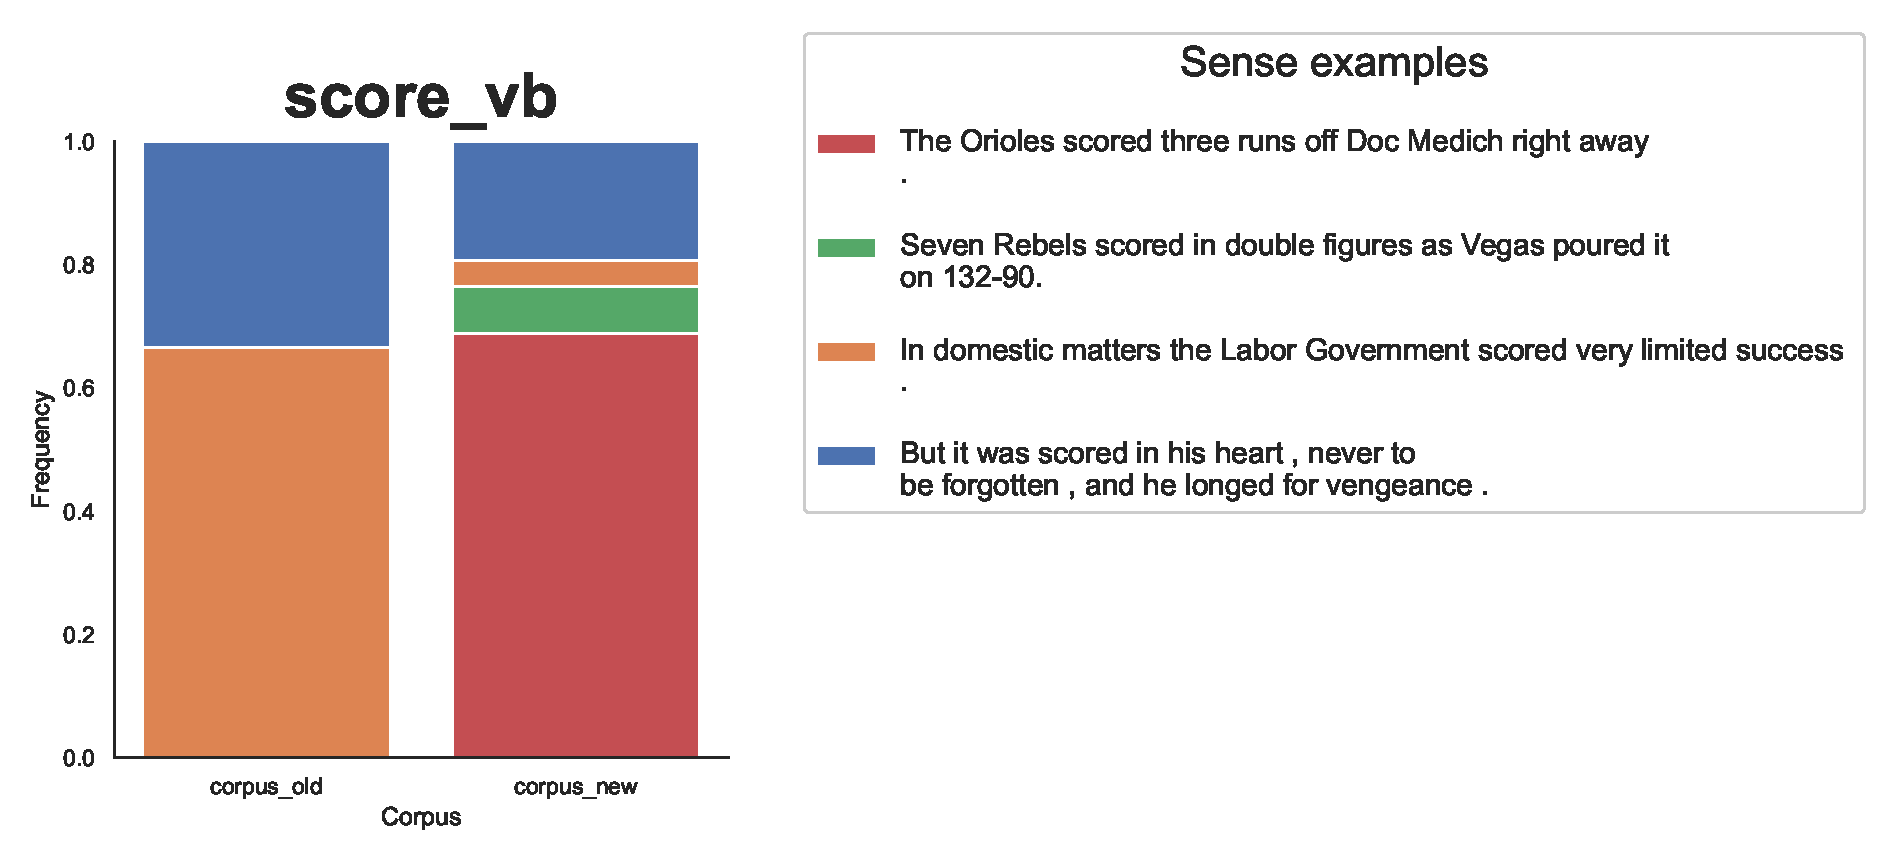
\includegraphics[width=0.65\textwidth]{img/33_score_vb.eps}
    
\end{frame}

\section{Historical Event Extraction}

\begin{frame}{Task Overview}
    \begin{itemize}
        \item \textbf{Objective}
        \begin{itemize}
            \item Detect historical events in a text
            \item Extract event arguments: dates, historical figures, locations
            \item Evaluate on Wikipedia pages  
        \end{itemize} 
        \item \textbf{Definition of historical events and entities}
        \begin{itemize}
            \item Events and entities that may be featured in a history textbook 
        \end{itemize}
        \item \textbf{Histo Corpus issues}
        \begin{itemize}
            \item Annotated events are not “historical"
            \item Different language from Wikipedia
            \item Event arguments are not annotated   
        \end{itemize} 
    \end{itemize}
\end{frame}

\begin{frame}{Data Sets}
    \begin{itemize}
        \item \textbf{RAMS Data Set (2020)}
        \begin{itemize}
            \item 139 event types
            \item up to 5 arguments per event
            \item 5 sentences and 1 event per document
            \item arguments cross event sentence boundaries 
        \end{itemize}
        
        \item \textbf{Wikipedia Data Set}
        \begin{itemize}
            \item 1024 pages
            \item pages, paragraphs and linked entities classified as historical or not based on Wikidata
            \item 16075 historical paragraphs and 23673 non-historical paragraphs 
            \item linked entities annotated in the BIO format 
        \end{itemize}

        \item \textbf{Linked entities are not enough for classification}
        \begin{itemize}
            \item only the first mention is linked
            \item surface form of an entity can vary greatly
        \end{itemize} 
        
    \end{itemize}
\end{frame}

\begin{frame}{Proposed Methods}
\center
    \includegraphics[width=0.9\textwidth]{img/event_strategy.png}
    \vspace{-10pt}
    \begin{itemize}
        \item \textbf{Paragraph classification} 
        \begin{itemize}
            \item a multi-task model (MTL) to jointly learn the class of the paragraph and the tag of the entities
        \end{itemize} 
        \item \textbf{Event extraction}
        \begin{itemize}
            \item enumerate spans and obtain span embeddings using BERT
            \item use a FFNN to classify each span and find the event “trigger"
        \end{itemize}  
        \item \textbf{Argument extraction}
        \begin{itemize}
            \item retrieve a pre-defined template for the identified event with “<arg>" placeholders
            \item let BART fill the placeholders by providing the text of the paragraph (Conditional Text Generation)
        \end{itemize} 
    \end{itemize}
\end{frame}

\begin{frame}[standout]
    Event: conflict.attack.invade \\
    \vspace{10pt}
    <arg> attacked <arg> using <arg> at <arg> place
\end{frame}

\begin{frame}{Results}
    \begin{table}
        \centering
        \resizebox{0.3\textwidth}{!}{
        \begin{tabular}{lcccc}
            \toprule
            Model & Acc & P & R & F1\\
            \midrule
            MTL & \textbf{84.2} & \textbf{80.6} & \textbf{84.2} & \textbf{82.4} \\
            BiLSTM & 74.4 & 74.7 & 74.4 & 74.5 \\
            BERT & 73.0 & 76.4 & 73.0 & 74.7 \\
            \bottomrule
        \end{tabular}
        }
    \end{table}

    \begin{table}
        \centering
        \resizebox{0.53\textwidth}{!}{
        \begin{tabular}{lccccccc}
            \toprule
            & \multicolumn{3}{c}{Events} & \multicolumn{3}{c}{Arguments} \\
            Model & P & R & F1 & P & R & F1\\
            \midrule
            Li et al. &  - & - & - & - & - & 48.6 \\
            Zhang et al. &  - & - & -  & - & - & 40.1 \\
            Zhang et al. (TCD)  & - & - & -  & - & - & 41.8 \\
            Wen et al.  & - & - & - & - & - & 48.6 \\
            Wei et al.  & - & - & - & 53.1 & \textbf{42.7} & 47.4 \\
            Lai et al.  & \textbf{71.9} & 74.7 & \textbf{73.2} & - & - & - \\
            Pouran Ben Veyseh et al.  & 55.5 & \textbf{78.6} & 65.1 & - & - & - \\
            Our BiLSTM baseline & 0.1 & 2.3 & 0.2 & - & - & - \\
            Our BERT baseline & 1.1 & 1.7 & 1.1 & - & - & - \\
            \textbf{Our model (EventGen)} & 29.8 & 27.9 & 24.8 & - & - & - \\
            \textbf{Our model} & 2.2 & 2.9 & 2.3 & \textbf{62.7} & 42.0 & \textbf{50.3} \\
            \bottomrule
        \end{tabular}
        }
    \end{table}
    
\end{frame}


\begin{frame}{Wikipedia Test Example}
    “In late 1941, Japan's government, led by Prime Minister and General Hideki Tojo, decided to break the US-led embargo \underline{through force of arms}. On December 7, 1941, the \underline{Imperial Japanese Navy} launched a surprise \underline{attack on the American fleet} at \underline{Pearl Harbor, Hawaii}. This brought the US into World War II on the side of the Allies. Japan then successfully \underline{invaded} the Asian colonies of the United States, the United Kingdom, and the Netherlands, including the Philippines, Malaya, Hong Kong, Singapore, Burma, and the Dutch East Indies."
    \begin{itemize}
        \item Predicted event: “conflict.attack.invade"
        \item Predicted arguments: “Imperial Japanese Navy attacked American fleet using arms at Pearl Harbor, Hawaii place"
    \end{itemize}
\end{frame}

\begin{frame}{Wikipedia Test Example}
    “In early 1944, towards the end of Tuker's time in Italy, during the Battle of Monte Cassino, \underline{Allied commanders} were engaged in a controversy regarding what action should be taken \underline{against the monastery at Monte Cassino}. The Germans had declared it a military-free zone but many senior commanders were reluctant to believe that the Germans would not occupy such a strategically important position. Tuker had found a book dated 1879 in a Naples bookshop giving details of the construction of the monastery at Monte Cassino which his division was to attack. He wrote a memorandum to his Corps commander, Lieutenant-General Bernard Freyberg, concluding that it should be demolished to prevent its occupation. He also pointed out that with 150-foot (45 m) high walls made of masonry at least 10 feet (3 m) thick, there was no practical means for field engineers to deal with the place, and that \underline{bombing with blockbuster bombs would be the only solution} since 1,000 pound bombs would be “next to useless". General Sir Harold Alexander, commanding the Allied Armies in Italy, \underline{agreed to the bombing (which did not employ blockbuster bombs)} and the ruins were occupied by German forces which held the position until 18 May."
    \begin{itemize}
        \item Predicted event: “artifactexistence.damagedestroy.destroy"
        \item Predicted arguments: “ Allied commanders destroyed monastery using blockbuster bombs instrument in Monte Cassino place"
    \end{itemize}
\end{frame}

\begin{frame}{Wikipedia Test Example}
    "After the Treaty of Versailles, treaties with Austria, Hungary, Bulgaria, and the Ottoman Empire were signed. However, \underline{the negotiation of the treaty with the Ottoman Empire} was followed by strife, and a final peace treaty between the \underline{Allied Powers} and the country that would shortly become the Republic of Turkey was not signed until 24 July 1923, \underline{at Lausanne} ."
    \begin{itemize}
        \item Predicted event: “government.agreements.unspecified"
        \item Predicted arguments: “Allied Powers and Ottoman Empire signed an agreement in Lausanne place"
    \end{itemize}
\end{frame}


\begin{frame}[standout]
    Thank You
\end{frame}

\begin{frame}[noframenumbering]{Wikipedia Test Example}
    “In June 2005, The Times newspaper alleged that Mladić had demanded a \$5 million (£2.75 million) “compensation" to be given to his family and bodyguards if he gave himself up to the ICTY in the Hague. In January 2006, \underline{a Belgrade court} indicted \underline{10 people for aiding Mladić} in hiding from 2002 to January 2006. An investigation showed \underline{Mladić spent his time in New Belgrade}, a suburb of the capital."

    \begin{itemize}
        \item Predicted event: “justice.initiatejudicialprocess.chargeindict"
        \item Predicted arguments: “court charged or indicted 10 people before  <arg>  court or judge for aiding Mladić crime in Belgrade place"
    \end{itemize}
\end{frame}

\end{document}
